
\documentclass[letterpaper,12pt,conference]{ieeeconf}

\IEEEoverridecommandlockouts
\overrideIEEEmargins

\usepackage{graphicx}
\usepackage{amsmath,amssymb}
\usepackage{bm}
\title{\LARGE \bf
Adaptive Traffic Signal Control Using
Demand Forecasting and Rolling-Horizon Optimization
}

\author{
Younggun Kim$^{1}$ and Manuel A. Martinez Garcia$^{1}$%
\thanks{$^{1}$Department of Civil and Environmental Engineering,
University of California, Los Angeles (UCLA),
Los Angeles, California, USA.}%
}

\begin{document}

\maketitle
\thispagestyle{empty}
\pagestyle{empty}

%%%%%%%%%%%%%%%%%%%%%%%%%%%%%%%%%%%%%%%%%%%%%%%%%%%%%%%%%%%%
\begin{abstract}

Traffic signal control plays an important role in managing
congestion and reducing vehicle delays at urban intersections.
Traditional fixed-time signal controllers rely on predetermined
timing plans that may not adequately respond to fluctuations
in traffic demand. While adaptive controllers can respond to
observed vehicle queues, they do not necessarily incorporate
recurring temporal patterns or uncertainty in future arrivals.
This project proposes a predictive traffic signal control framework that integrates Transformer-based traffic demand forecasting with rolling-horizon optimization. The forecasting model learns temporal demand patterns from historical vehicle arrivals and time-of-day information to predict traffic demand over a finite future horizon. These predictions are incorporated into a rolling-horizon optimization component that dynamically determines signal phases and green time allocations to minimize cumulative vehicle delay subject to operational constraints.
Using an isolated-intersection simulation,
we will compare the proposed controller against fixed-time
and queue-responsive control under balanced demand,
directional demand shifts, heavy congestion, and imperfect
detector observations. We will evaluate whether incorporating
forecasts improves traffic signal performance and
investigate how forecasting errors affect control decisions.

\end{abstract}

%%%%%%%%%%%%%%%%%%%%%%%%%%%%%%%%%%%%%%%%%%%%%%%%%%%%%%%%%%%%
\section{INTRODUCTION}

Traffic congestion at signalized intersections remains a
significant challenge in urban transportation systems, often
contributing to increased travel times, vehicle delays, and
inefficient utilization of roadway capacity. Conventional
fixed-time traffic signal controllers allocate green time
according to predetermined schedules, typically designed
around representative traffic demand conditions. Although
these controllers are relatively simple to implement,
their performance may deteriorate when actual traffic
conditions deviate from the assumptions used to develop
their timing plans. Adaptive traffic signal control provides
an alternative by adjusting signal timings in response to
observed traffic conditions, potentially improving traffic
flow and reducing delays.


\begin{figure}
    \centering
    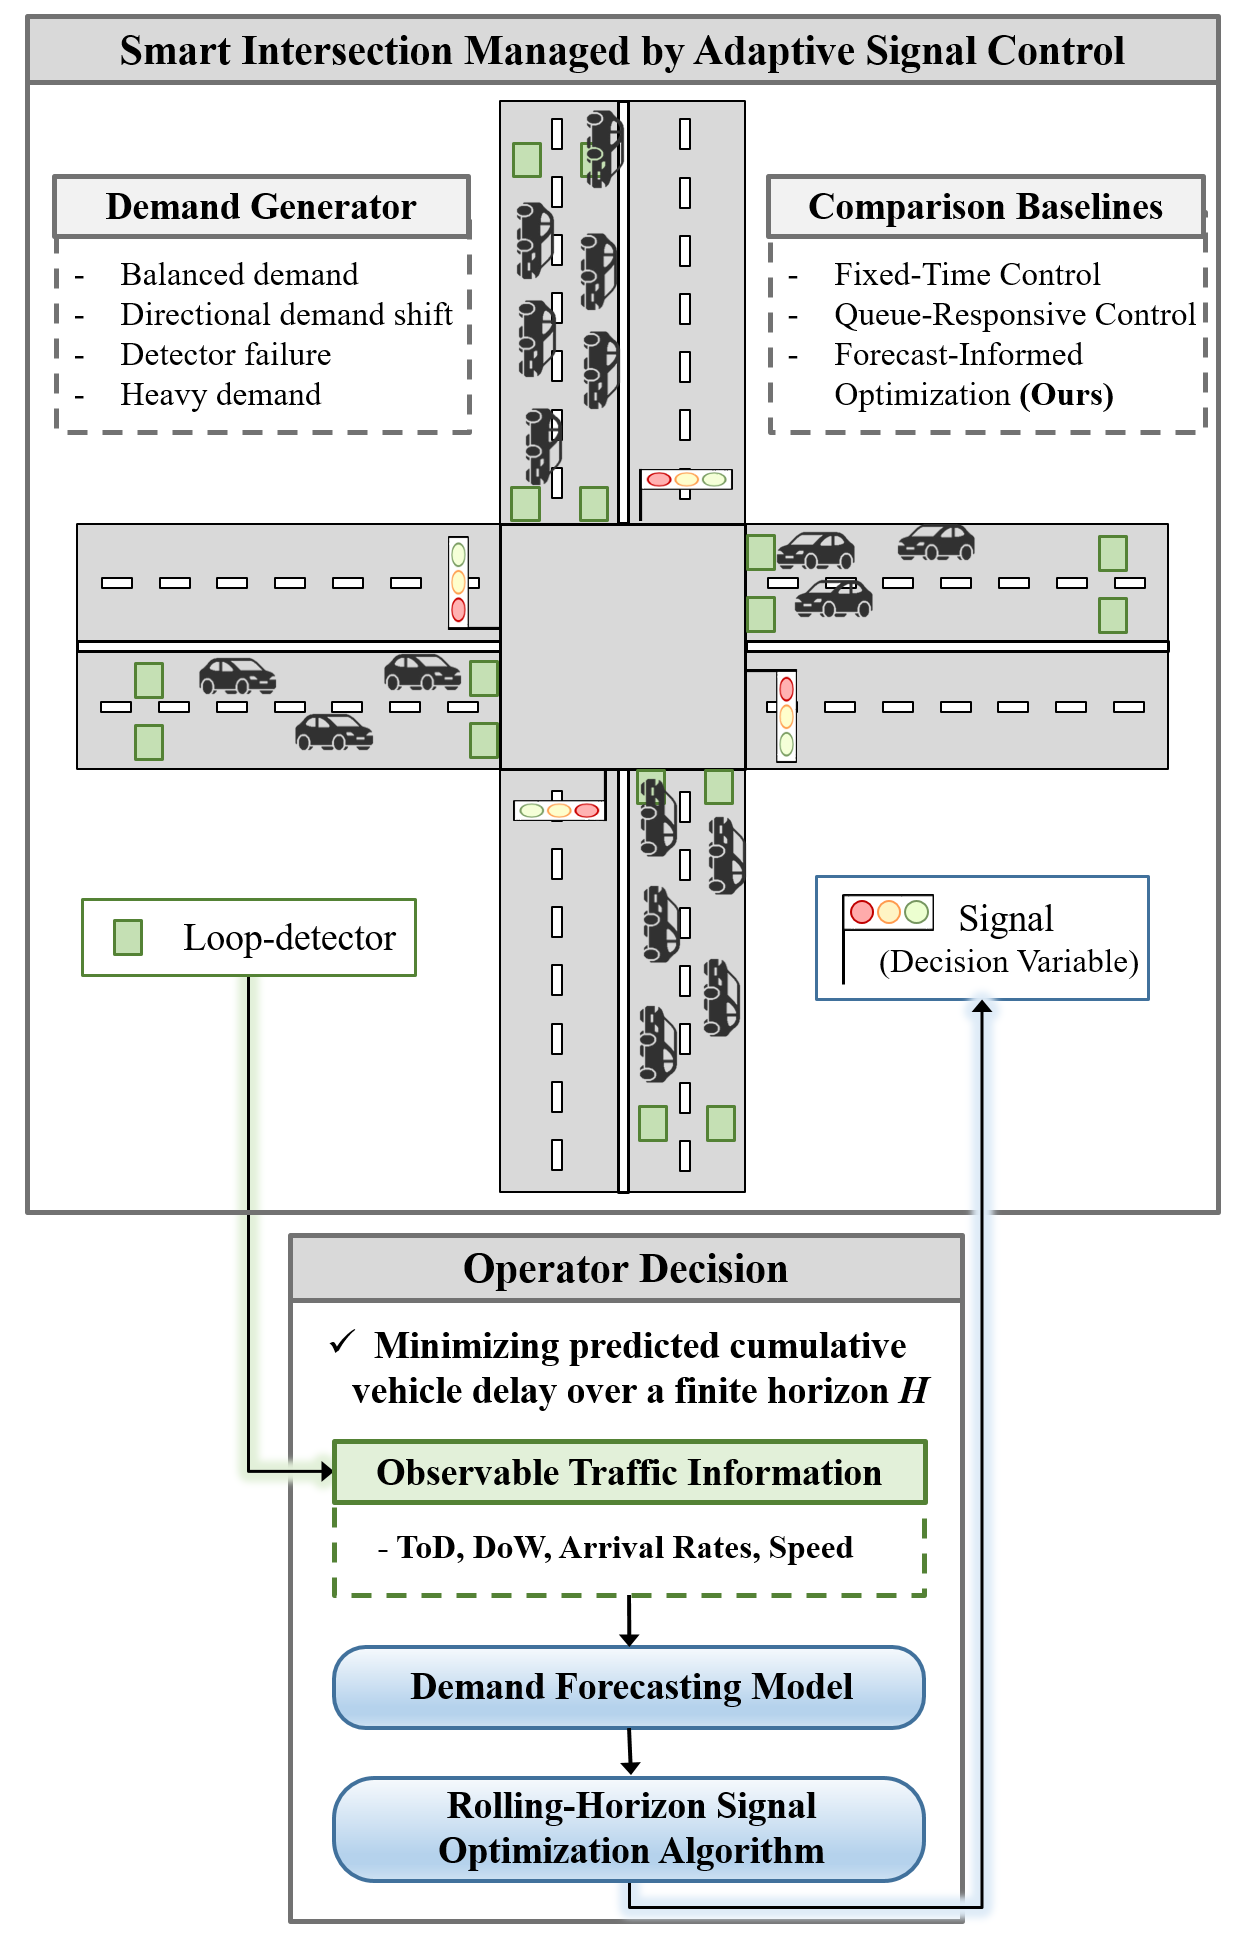
\includegraphics[width=\linewidth]{System_Illustration.png}
    \caption{Overview of the proposed adaptive traffic signal control framework integrating Transformer-based demand forecasting and rolling-horizon optimization in an isolated intersection.}
    \label{fig:System_Illustration}
\end{figure}

One important characteristic of traffic demand is its
temporal variability. Traffic arrivals often exhibit
recurring patterns associated with time of day and day of
the week. Recent research
by ElKhouly et al. \cite{elkhouly2025} demonstrates the
potential of forecasting methods to capture
multiple demand patterns in intersection traffic volumes.
Additionally, Li and Savla \cite{li2025} investigate
adaptive model predictive control for traffic signal timing
under unknown traffic demand and system parameters.
More recently, Atef and Karam \cite{atef2026} combined
traffic forecasting with constrained model predictive
control to address recurring changes in demand.

These studies highlight the potential of integrating
predictive information with optimization-based traffic
signal control. However, an important question remains
regarding how much demand forecasting improves actual
control performance, particularly when observed traffic
conditions deviate from historical patterns or measurements
become unreliable.



In this project, as illustrated in Figure~\ref{fig:System_Illustration}, we propose developing an
adaptive traffic signal controller that combines demand
forecasting with rolling-horizon optimization. Our approach
will estimate short-term traffic arrivals using recurring
demand patterns and continuously update these predictions
using available detector observations. The resulting
forecasts will inform an optimization model that determines
feasible green time allocations while considering vehicle
queues, discharge capacities, minimum and maximum green
times, and phase-transition requirements.

We will implement the proposed framework using the provided
isolated-intersection simulation scaffold and compare its
performance against justified fixed-time and queue-responsive
controllers. Through simulation experiments involving
changing traffic demand, heavy congestion, and detector
failures, we aim to investigate the relationship between
forecasting accuracy and traffic signal performance, with
particular emphasis on total intersection delay, throughput,
queue lengths, and service imbalance across approaches.

%%%%%%%%%%%%%%%%%%%%%%%%%%%%%%%%%%%%%%%%%%%%%%%%%%%%%%%%%%%%
\section{PROPOSED METHODOLOGY}

Our proposed framework consists of three main components:
demand traffic forecasting, rolling-horizon signal
optimization, and simulation-based performance evaluation.

\subsection{Intersection Model}

We consider an isolated four-way signalized intersection
consisting of northbound, southbound, eastbound, and
westbound approaches.

For simplicity, the initial model will consider two
compatible traffic signal phases:

\begin{itemize}
    \item Phase 1: Northbound and southbound through movements.
    \item Phase 2: Eastbound and westbound through movements.
\end{itemize}

Vehicle arrivals, queue formation, and stop-line discharge
will be represented using the provided simulation scaffold.
The initial scope excludes pedestrian movements and turning
movements.

Signal operation will satisfy minimum and maximum green
durations, yellow and all-red clearance intervals,
movement compatibility, and discharge capacity constraints.







\subsection{Transformer-Based Traffic Demand Forecasting}

We propose a Transformer-based forecasting model to
predict short-term vehicle arrival rates using historical
traffic observations and temporal information.

Let $\mathcal{A}$ denote the set of intersection
approaches, and let $\boldsymbol{\lambda}_t$ denote
the vector of observed arrival rates at time $t$.

At each prediction time $t$, the model takes a historical
sequence of length $L$ as input:

\begin{equation}
\mathbf{X}_t =
[
\boldsymbol{\lambda}_{t-L+1},
\ldots,
\boldsymbol{\lambda}_t
].
\end{equation}

The historical demand sequence is augmented with
time-of-day (ToD) and day-of-week (DoW) features
to capture recurring temporal patterns.

The Transformer, parameterized by $\theta$, predicts
the vehicle arrival rate for each approach $i$
at the next time step:

\begin{equation}
\hat{\lambda}_{i,t+1}
=
f_{\theta}(\mathbf{X}_t,\mathbf{C}_t)_i,
\qquad i \in \mathcal{A},
\end{equation}

where $\mathbf{C}_t$ contains the corresponding
ToD and DoW features.

To obtain forecasts over a future horizon $H$,
the predicted arrival rates are recursively fed
back into the historical input sequence.
At each iteration, the oldest observation is removed
and the latest prediction is appended along with
its corresponding temporal features.
This process is repeated $H$ times using the
same Transformer model.


The resulting demand forecasts will be incorporated
into the rolling-horizon signal optimization model
to determine future signal control decisions.





\subsection{Rolling-Horizon Signal Optimization}

The estimated arrival rates will be incorporated into a
rolling-horizon optimization framework that determines
future signal phases and green time allocations.

Let $q_{i,t}$ represent the queue length at approach $i$
and time $t$. The queue dynamics may be represented by

\begin{equation}
q_{i,t+1}
=
q_{i,t}
+
a_{i,t}
-
d_{i,t},
\end{equation}

where $a_{i,t}$ denotes accepted vehicle arrivals and
$d_{i,t}$ denotes the number of discharged vehicles.

For finite-storage approaches, arrivals that cannot enter
the intersection model will be recorded as unmet demand
rather than discarded.

The optimization objective will seek to minimize predicted
cumulative vehicle delay over a finite horizon $H$.

A preliminary objective can be expressed as

\begin{equation}
\min_{\mathbf{u}}
\mathbb{E}
\left[
\sum_{\tau=t}^{t+H-1}
\sum_{i \in \mathcal{A}}
q_{i,\tau}\Delta t
\right],
\end{equation}

where $\mathbf{u}$ represents feasible signal control decisions
and $\Delta t$ is the simulation time step.

The cumulative queue term serves as a measure of total
vehicle waiting time. Additional penalties may be
introduced to discourage excessive service imbalance
between approaches.

The optimization will enforce signal phase compatibility,
minimum and maximum green times, clearance intervals,
and vehicle discharge constraints.

At each decision interval, the controller will implement
the first feasible control decision, update its observations,
and repeat the optimization process.

%%%%%%%%%%%%%%%%%%%%%%%%%%%%%%%%%%%%%%%%%%%%%%%%%%%%%%%%%%%%
\section{SIMULATION AND EVALUATION}

\subsection{Controller Comparison}

We propose evaluating three traffic signal control
strategies:

\begin{enumerate}

    \item Fixed-Time Control:
    A predetermined signal timing plan calibrated to
    representative traffic demand.

    \item Queue-Responsive Control:
    A controller that adjusts signal decisions based
    on observed vehicle queues.

    \item Forecast-Informed Optimization:
    A rolling-horizon controller that incorporates
    demand forecasts and updated traffic
    observations.

\end{enumerate}

All controllers will operate under the same signal
phase and clearance constraints to ensure a fair
comparison.

\subsection{Simulation Scenarios}

We will evaluate controller performance under four
traffic conditions:

\begin{enumerate}

    \item Balanced demand:
    Comparable arrival rates across intersection
    approaches.

    \item Directional demand shift:
    A sudden increase in vehicle arrivals along
    one intersection direction.

    \item Detector failure:
    Missing, inaccurate, or delayed observations
    of traffic conditions.

    \item Heavy demand:
    Arrival rates approaching or exceeding
    available intersection service capacity.

\end{enumerate}

When observations become unreliable, the proposed
controller will apply a predefined fallback timing plan.

All experiments will use identical demand realizations,
initial queues, and simulation horizons across controllers.

\subsection{Performance Metrics}

Controller performance will be evaluated using:

\begin{itemize}
    \item Total and approach-specific vehicle delay.
    \item Intersection throughput.
    \item Maximum and residual queue lengths.
    \item Unmet vehicle demand.
    \item Service imbalance between approaches.
\end{itemize}

We will also examine signal phase timelines and the
corresponding queue evolution to verify the controller's
behavior and signal transition constraints.

\subsection{Statistical Analysis}

Repeated simulation experiments will be conducted using
different random seeds to capture variability in vehicle
arrivals.

We will compare controller performance using paired
experimental observations, summary statistics, and
confidence intervals.

Additionally, we propose conducting a sensitivity study
to investigate how forecast accuracy and observation delays affect optimization performance.

An ablation experiment may compare the same optimization
controller with and without seasonal forecasting to
isolate the contribution of the statistical model.

%%%%%%%%%%%%%%%%%%%%%%%%%%%%%%%%%%%%%%%%%%%%%%%%%%%%%%%%%%%%
\section{EXPECTED CONTRIBUTIONS}

The primary objective of this project is to investigate
the benefits and limitations of incorporating demand
traffic forecasting into adaptive traffic signal control.

We aim to evaluate whether the predicted traffic information
improves short-term signal decisions relative to
conventional fixed-time and queue-responsive controllers.

Additionally, we seek to understand how forecasting
errors and unreliable observations influence optimization
performance under changing traffic conditions.

The results may help identify circumstances in which
forecast-informed optimization provides measurable
benefits and circumstances in which simpler traffic
signal control strategies remain competitive.

If successful, this work could demonstrate the potential of forecast-informed traffic signal control at intersections where sufficient historical and real-time traffic data are available, potentially reducing traffic delays and improving overall intersection efficiency.

%%%%%%%%%%%%%%%%%%%%%%%%%%%%%%%%%%%%%%%%%%%%%%%%%%%%%%%%%%%%
\begin{thebibliography}{99}

\bibitem{atef2026}
S. Atef and A. Karam,
``An Adaptive Traffic Signal Control Framework
Integrating Regime-Aware LSTM Forecasting and Signal
Optimization Under Socio-Temporal Demand Shifts,''
\textit{Applied System Innovation},
vol. 9, no. 4, art. 81, 2026.
doi: 10.3390/asi9040081.

\bibitem{elkhouly2025}
M. ElKhouly, T. Alhadidi, and H. Rakha,
``Modeling Traffic Vehicular Counts at an Urban
Intersection Using Complex Seasonal Modeling Techniques,''
\textit{KSCE Journal of Civil Engineering},
vol. 29, no. 1, art. 100040, 2025.
doi: 10.1016/j.kscej.2024.100040.

\bibitem{li2025}
Z. Li and K. Savla,
``Adaptive Model Predictive Control for Traffic Signal
Timing with Unknown Demand and Parameters,''
arXiv:2503.10934, 2025.

\bibitem{jia2025}
S. Jia, S. C. Wong, and W. Wong,
``Adaptive Signal Control at Partially Connected
Intersections: A Stochastic Optimization Model for
Uncertain Vehicle Arrival Rates,''
\textit{Transportation Research Part B: Methodological},
vol. 193, art. 103161, 2025.
doi: 10.1016/j.trb.2025.103161.

\bibitem{varaiya2013}
P. Varaiya,
``Max Pressure Control of a Network of Signalized
Intersections,''
\textit{Transportation Research Part C:
Emerging Technologies},
vol. 36, pp. 177--195, 2013.
doi: 10.1016/j.trc.2013.08.014.

\bibitem{signalmanual2015}
National Academies of Sciences, Engineering, and Medicine,
\textit{Signal Timing Manual -- Second Edition}.
Washington, DC: The National Academies Press, 2015.
doi: 10.17226/22097.

\end{thebibliography}

\end{document}
